\documentclass[12pt]{article}
\usepackage[margin=1.0in]{geometry}
\usepackage{setspace}
\usepackage{indentfirst}
\usepackage{array}
%\usepackage{longtable}
\usepackage{graphicx}
\graphicspath{ {diagrams/} }

\usepackage[T1]{fontenc}
\usepackage[default]{raleway}

\usepackage[stable]{footmisc}


\PassOptionsToPackage{hyphens}{url}\usepackage{hyperref}

\title{Endrun---Secure Digital Communications For Our Modern Dystopia\footnote{This paper, and the work it describes, represents the work of the authors in their spare time, and represents neither the product, nor the policy, of either author's employer(s). Conclusions of law in this work are not ``legal advice,'' do not establish an attorney-client relationship, and may be neither sane nor coherent.}}
\author{Grant Dobbe\footnote{Lead Security Engineer and Cloud Services Meteorologist, NuCivic Inc.}\space\space and Brendan O'Connor\footnote{Senior Security Consultant, Leviathan Security Group}}
\date{October 16, 2014}

\begin{document}
	
	\maketitle
  
  \begin{quote}
    \emph{The Internet is no longer trustworthy, having been compromised by bad actors across the globe. Current proposals to work around a compromised Internet rely upon encrypted transport links, mesh networks, or harassing users for being unable to use GPG safely. Each of these strategies fails in different ways that inevitably lead to information leakage or---in the extreme case---death. Endrun, by contrast, takes NASA's Disruption-Tolerant Networking project from a laboratory experiment to a functional system that supports user-friendly encryption in hostile environments. Endrun embraces the nearly-unlimited throughput of a disk-laden station wagon and creates a reliable, eventually-consistent communications system ideal for activists, refugees, and trolls.}
    \end{quote}
	
	\section{Introduction}
	
  It's easy to speak when everyone loves you. When people in the US or the rest of the western world discuss ``free speech,'' they generally mean some form of the right to communicate with others, and to assemble with others for the purpose of sharing their message. Some may also refer to a right to anonymous speech, but there are those who would attack the right of anonymity; ``if you have nothing to hide, you have nothing to fear.''\footnote{For an excellent response to this common fallacy, see ``Why Privacy Matters Even if You Have `Nothing to Hide,'\,'' Daniel J. Solove, The Chronicle of Higher Education, May 15, 2011 \url{https://chronicle.com/article/Why-Privacy-Matters-Even-if/127461/}.} In an era when ``privacy is dead, get over it''\footnote{Stated by many, including Sun Microsystems' Scott McNealy; \url{http://archive.wired.com/politics/law/news/1999/01/17538}}, it's easy to say that ``Users who try to use anonymity, or cover themselves up on the internet, are usually doing things that aren`t so-to-speak legal.''\footnote{Attributed to Comcast, who has since denied holding this position. \emph{See} ``Comcast Denies It Will Cut Off Customers Who Use Tor, The Web Browser For Criminals,'' James Cook, Business Insider, September 15, 2014, \url{http://www.businessinsider.com/comcast-threatens-to-cut-off-tor-users-2014-9}}
  
  We dissent. The right of public speech was not created to protect those messages everyone loves, but those messages that are reviled (for whatever reason). We believe that the current age of ``registered bloggers''\footnote{See, for example, Russia's new law. \url{https://www.techdirt.com/articles/20140423/09130227004/russian-net-clampdown-continues-now-its-turn-blogs-vkontakte.shtml}} and believing that press members are only real if they have a ``\$50,000 camera''\footnote{``Ferguson Police Say They May Arrest More Journalists,'' Jack Mirkinson, The Huffington post, August 19, 2014, \url{http://www.huffingtonpost.com/2014/08/19/ferguson-police-arresting-journalists_n_5691645.html}} reflects a misguided and destructive impulse to control thought and expression for the sake of centralization of power. We therefore present a system that we intend to provide a useful counterbalance; an easy-to-use, strongly-encrypted information-sharing network built not upon a reliable Internet source, but upon the distributed, unending movements of people. 
  
  \begin{quote}
    \emph{You may stop this individual, but you can't stop us all... after all, we're all alike.}\footnote{``The Conscience of a Hacker,'' The Mentor, Phrack, Volume One, Issue 7, Phile 3 of 10 (Written January 8, 1986; Published September 25, 1986)}
  \end{quote}
  
  \section{Design Goals for Endrun}
  
  Endrun has five major design goals.
  
  \begin{enumerate}
    \item Endrun is designed to make an ``end run'' around the Internet, for the purpose of giving a communications option to people who cannot use the Internet. This could happen for any of several reasons: the Internet could have suffered a major regional or global failure, due to natural disaster, accident, or hostility; the Internet might be considered untrustworthy, due to adversary action; or the areas being communicated across might be so remote that Internet connectivity is simply not a useful option.\footnote{While a large portion of the planet is served at least by bidirectional satellite Internet service, if nothing else, such service is often overwhelmingly expensive for all but the largest corporations, and this service does not reach the entire planet.}
    
    \item Endrun is designed for communications between small groups of people---``cells'' or ``pods.'' It is not designed for open-ended communication between people that have no prior relationship.
    
    \item Endrun is ``by any means necessary.'' Endrun is designed to work across any form of communication that is available, whether that's physical data movement and low-power transient unlicensed radio links, as we would recommend, or by Earth-Moon-Earth (EME) high-powered signals from fix points, or even amateur (ham) radio.\footnote{This use of amateur radio would almost certainly be illegal in many countries for several reasons, among them Endrun's use of multiple layers of strong encryption, and the fact that messages may not necessarily be originated by ham radio stations.}
    
    \item Endrun is disruption- and delay-tolerant. It is designed to work where nodes have no real- or bounded-time connection to each other, for instance, when couriers are moving data stored on physical media either around town or across a continent.
    
    \item Endrun is built using standard, well-tested, open source components and combined using Python, rather than using all custom code. This lets Endrun benefit from decades of work from thousands of programmers (with all the attendant work on security that implies). It also means that Endrun is customizable by programmers in the field; in an emergency situation, this can give flexibility that fully-custom solutions cannot.
    
  \end{enumerate}
  
  \section{Previous Work}
  \label{sec:previouswork}
  
  There has been a great deal of interest in the area of distributed communication tools, both ones that work over the public Internet, and ones that establish their own wireless links. We will examine several of the largest and most influential projects.
  
  \subsection{Tor}
  
  Tor\footnote{\url{https://www.torproject.org}} is an incredibly-well-known tool for anonymous Internet access. The core security concept of Tor is called ``onion routing,'' where a client picks several nodes to pass the client's message through, and repeatedly encrypts the message with the public key of each node; the message is then routed in turn through each node. This means that if a client picks nodes A, B, and C to transit the message through, in that order, then node A knows where the message originated but not where it is destined (nor its contents), node C knows the message's destination and contents (assuming that no additional encryption is used), but not where it originated, and node B knows neither the message's contents, nor its source, nor its destination.
  
  Tor was originally developed by the U.S. Naval Research Laboratory, subsequently developed by the Defense Advanced Research Projects Agency, and then transferred for ongoing development to The Tor Project, a U.S.-based nonprofit corporation. It is rightly lauded as one of the most important security projects since the invention of networked computing; that said, it has certain deficits which raise concerns for anonymity applications. One of these is that when an adversary is able to monitor both the source and destination networks of a Tor message, a trivial timing analysis will reveal which user sent which message. This was revealed very dramatically through the near-instantaneous reidentification and arrest of Eldo Kim after he used Tor to send a bomb threat to Harvard University, which he attended at the time, apparently to escape a final exam.\footnote{``Harvard Student Receives F For Tor Failure While Sending `Anonymous' Bomb Threat,'' Runa A.\ Sandvik, Forbes, December 18, 2013, \url{http://www.forbes.com/sites/runasandvik/2013/12/18/harvard-student-receives-f-for-tor-failure-while-sending-anonymous-bomb-threat/}} Another, related, issue is that if an adversary controls a significant percentage of the total Tor network, they will nearly always be able to identify both the source and destination of any message (through a timing analysis of any message that both enters and leaves the Tor network through the adversary's systems). Both of these problems were noted in the original Tor paper.\footnote{``Tor does not claim to completely solve end-to-end timing or intersection attacks.'' Page 4 of ``Tor: The Second-Generation Onion Router,'' Roger Dingledine, Nick Mathewson, Paul Syverson, Proceedings of the 13th USENIX Security Symposium, 2004, \url{https://www.usenix.org/legacy/events/sec04/tech/full_papers/dingledine/dingledine.pdf}} At the time, however, it was believed that increased Tor usage, with an attendant increase in Tor nodes, would render controlling a majority of machines impractical.
  
  Unfortunately, this assumption is now believed to be incorrect. Tor's public metrics\footnote{\url{https://metrics.torproject.org/network.html}} indicate the daily average number of nodes is approximately 6,000 (as of September 2014). An adversary could match that number of nodes (and thus control 50\% of the total nodes on the network) relatively cheaply; using Amazon Web Services On-Demand Micro Instances, 6,000 nodes would cost just \$56,160 per month to operate (plus bandwidth).\footnote{Pricing data from \url{http://aws.amazon.com/ec2/pricing/}.} An adversary with a relatively small datacenter and sufficient bandwidth could spend significantly less on an ongoing basis to compromise the Tor network, and there are allegations that certain entities have already done so. We believe that Tor is now insufficient for truly-suppressed parties to communicate anonymously in the face of a network-level adversary.
  
  \subsection{Anonymous AirChat}
  \label{subsec:airchat}
  
  Airchat\footnote{\url{https://github.com/lulzlabs/AirChat/}} was announced on April 23, 2014, to great fanfare, promising Internet-free end-to-end encrypted connection suitable for text and low-bandwidth digital voice communication over up to 100 miles, using simple radios. Airchat has the dubious distinction of stating an intent to use the system over amateur radio, on which encryption is forbidden (except in certain circumstances), and further stating that ``we dont give a fucking shit about prohibitions over the use of encryption. fuck you NSA. [sic]\footnote{\url{https://github.com/lulzlabs/AirChat/commit/1b289a8a46c7c25c419a8d2b9b761db13142e53d\#diff-c47c7c7383225ab55ff591cb59c41e6bR174}}'' Setting aside the question of an openly-stated conspiracy to violate U.S. regulations (among many other countries that prohibit encryption on amateur radio frequencies), AirChat seems reasonable. The downside, however, is that it is an online protocol; both sides are communicating continuously, and due to their use of fairly low-throughput protocols,\footnote{The default protocol for AirChat is PSK500R, providing 506 baud of throughput; since PSK500R uses binary keying, this means it is transmitting just 506 bits per second.} stations are communicating for a long time. The use of ham radios means that stations are also communicating using relatively high power,\footnote{An average ham radio ``Handie-Talkie,'' or HT, transmits at 5W out of the box; amateur radio operators in many countries may use up to 1500W of transmitting power.} which, when combined with the need to transmit for long periods of time in once place, means that stations can easily be located.
  
  If stations can be located easily, they can be destroyed very easily. It has been reported that Syria may have used missiles that track satellite phones to kill journalists.\footnote{``Caveat utilitor: Satellite phones can always be tracked,'' Frank Smyth, Committee to Protect Journalists, February 24, 2012, \url{http://cpj.org/blog/2012/02/caveat-utilitor-satellite-phones-can-always-be-tra.php}} One representative satellite phone, the Iridium Extreme 9575 Satellite Phone, transmits at approximately 250mW,\footnote{\url{https://apps.fcc.gov/eas/GetApplicationAttachment.html?id=1508135}} or 1/20th the transmit power of a typical cheap ham radio. This means a node running AirChat could face a missile even more easily than a satellite phone. Unfortunately, we believe that high-powered wireless links cannot be the basis of a system designed to protect anonymity in hostile areas, given this capability.
  
  \subsection{Commotion Wireless / Project Byzantium}
  
  Commotion Wireless\footnote{\url{https://commotionwireless.net}} and Project Byzantium\footnote{\url{http://project-byzantium.org}} represent two different ideas in mesh WiFi. Commotion is designed to be installed to consumer WiFi routers, providing mesh connectivity that can give wireless Internet access to neighborhoods; Byzantium describes itself as ``Ad-hoc wireless mesh networking for the zombie apocalypse,'' and provides software to turn consumer laptops into mesh nodes that provide communication services without Internet access. While both projects are of course admirable, they necessarily fall victim to the same problem discussed in Section~\ref{subsec:airchat}: long-lived, fixed wireless transmitters are dangerous for environments of censorship. (The hypothetical zombie apocalypse might be an acceptable time for use of these systems, however, since zombies are unlikely to employ automatic direction finding technology, or missiles, according to standard reference sources.\footnote{\emph{See, e.g.,} Zombieland (2009), Day of the Dead (1985), or Plan 9 from Outer Space (1959).}
  
  \subsection{Delay-Tolerant Networking}
  \label{subsec:dtn}
  
  The concept of delay- or disruption-tolerant networking has been the subject of a great deal of research, both by NASA, in the context of Vint Cerf's Interplanetary Networking (IPN) proposals,\footnote{\url{http://ipnsig.org}} and by DARPA-funded researchers looking for land-based solutions.\footnote{\url{https://www.fbo.gov/index?s=opportunity&mode=form&id=9e7abdcb0d96df48de122b0ec28e96d1&tab=core&_cview=0}} The concept is the same, with minor differences in application; both groups want to enable networked communication between nodes that may not be able to support bidirectional end-to-end communication, either due to vagaries of remote terrain (for DARPA), or light-speed communications delays across the solar system (for NASA). This is achieved through store-and-forward routing, with opportunistic data transmission when nodes indicate that they
  
  The DTN concept is perfect in many ways for decentralized communication between marginalized groups; the current implementations, however, leave much to be desired. There is no common implementation of DTN; rather, there are several different codebases, such as DTN2\footnote{\url{http://sourceforge.net/project/showfiles.php?group_id=101657}}, ION\footnote{\url{https://ion.ocp.ohiou.edu/}}, and IBR-DTN\footnote{\url{http://www.ibr.cs.tu-bs.de/trac/ibr-dtn}}, none of which are considered by their authors to be either complete or stable. The DTNBone project\footnote{\url{https://sites.google.com/site/dtnresgroup/home/dtn-bone}} catalogues the efforts being made to create a continuously operating DTN network in academia. NASA, too, has failed to create a DTN network; while several DTN-capable payloads have been launched, other projects necessary to establish a true interplanetary link were scrapped due to ``sequestration'' and other budgetary cuts.
  
  The DTN protocol as currently designed suffers from other problems. Message security is an optional add-on layer, rather than being a core part of the protocol. The binary protocol is highly complex and requires a parser to conditionally process different parts of the bundle depending on earlier flags,\footnote{See IETF RFC 5050, \url{http://tools.ietf.org/html/rfc5050}} meaning that parsing protocols must be at least context-sensitive.\footnote{This is undesirable for security functions; for more information, see the work of the Language-theoretic Security Working Group (Patterson, Hirsch, Bratus, Goodspeed, Sassaman, Shubina, et al) at \url{http://langsec.org}.} While the DTN concept is highly desirable, then, the implementation is not usable in the field at this time.
  
  \section{Method}
  
  As noted in Section~\ref{subsec:dtn}, we believe the concept of DTN, with store-and-forward routing with opportunistic sending, is great for disconnected parties wishing to communicate without Internet access, but the specific protocol is difficult to work with and has security as an afterthought---and even if it were perfect for our needs, no stable implementations exist. We have therefore implemented our own version of the DTN protocol. The following sections will describe how each major Endrun component works.
  
  \subsection{Routing}
  \label{subsec:routing}
  
    Delay-Tolerant networking, like TCP/IP, assigns an address to each node in a network, and passes traffic between nodes via whatever route is available. Unlike TCP/IP, however, DTN nodes do not engage in any sort of handshake to exchange data in an end-to-end fashion; instead, each sequential pair of nodes in a communication pathway exchange data and sign a chain of custody showing that they successfully received and have taken responsibility for the data.
    
    Data may take any available path between a pair of nodes in a chain; it might use physical data transport (sneakernet), a radio link, or anything else that is available (including TCP/IP, where that is possible). The crucial difference is that there is no expectation that the source and destination node will be communicating simultaneously at any point; instead, only pairs in the chain will communicate.
    
    \begin{figure}[h]
      \centering
      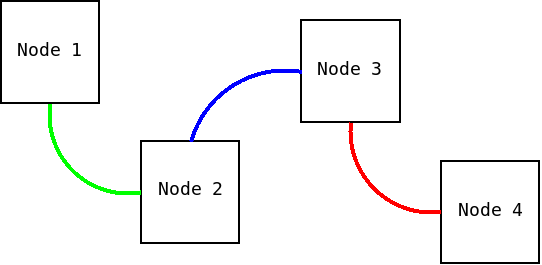
\includegraphics[scale=0.5]{Diagram1.png}
      \caption{An example of how nodes can transmit data. In this example, there is no direct path between Node 1 and Node 4; Node 2 and Node 3 are used to relay the information.}
    \end{figure}
    
    Because links between nodes are transient, our implementation of DTN does not use anything resembling a traditional routing table. Instead, it uses the ``binary spray and wait'' transmission strategy.\footnote{Thrasyvoulos Spyropoulos, Konstantinos Psounis, and Cauligi S. Raghavendra. Spray and wait: An efficient routing scheme for intermittently connected mobile networks. In WDTN '05: Proceeding of the 2005 ACM SIGCOMM workshop on Delay-tolerant networking, 2005.} Binary spray and wait allows for the transmission of data with minimal delay and highest efficiency with regards to network traffic, while still allowing for transience in connectivity.
    
    Binary spray-and-wait sets a ceiling on the number of payload copies \(L\) that can exist within the network. When a payload is being sent, the originating node starts in ``spray'' mode, where it transmits a copy of the payload to \(floor(L/2)\) nodes; each subsequent node then transmits half of their total payload copies to every other node without a copy of the payload. When a node has 1 copy of the message remaining, it switches to ``wait'' mode, where it holds a copy of the payload until either it makes direct contact with the recipient node or the TTL is reached.
    
    \begin{figure}[h]
      \centering{}
      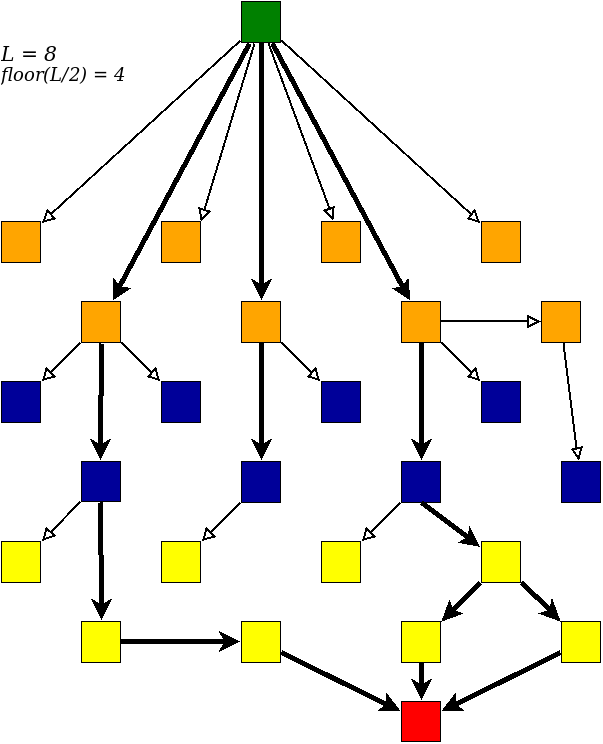
\includegraphics[scale=0.45]{Diagram2.png}
      \caption{An example of how nodes distribute copies of a payload using the binary spray-and-wait strategy.}
    \end{figure}
    
  \subsection{User Services}
  
  The services provided to users within Endrun are fairly simple. In addition to transport-related services, discussed in Section~\ref{subsec:transport}, users have access to Gollum,\footnote{\url{https://github.com/gollum/gollum}}, a Git-based wiki. The wiki provides standard text-based services, and also supports file uploads.
  
  On top of Gollum, then, users can implement any of the following that are desired:
  \begin{itemize}
    \item Encrypted user-to-user messaging, using GPG or another encryption system.
    \item Forum/bulletin board functionality, using the wiki directly.
    \item Encrypted file transfer, using, e.g., Minilock\footnote{\url{https://minilock.io}} or another simple encryption system
  \end{itemize}
  
  These services allow the basic use case---allowing communications between pods of people unable to use the general Internet---to take place, without adding excessive complexity.
  
  \subsection{Message Format}
  
  The Endrun payload message format is designed to be very simple to parse. It has the following fields:
  
  \begin{enumerate}
    \item \textbf{\textsc{Source}} - The identifier for the source node.
    \item \textbf{\textsc{Destination}} - The identifier for the destination node.
    \item \textbf{\textsc{TTL}} - The message time to live, an integer number representing the epoch time at which the bundle was created. Nodes destroy messages after a configurable amount of time has passed since their creation (by default, 24 hours).
    \item \textbf{\textsc{Contents}} - The signed, then encrypted, then signed message bundle.
    \item \textbf{\textsc{Chain of Custody}} - A JSON object detailing the transmission path of the payload. See Section~\ref{subsec:chainofcustody}: for more details.
    %\item \textbf{\textsc{Transmission Ceiling}} - The maximum number of copies of this payload that should exist per Section~\ref{subsec:routing}:.

    \end{enumerate}
    
    Payloads are encrypted with the libsodium implementation\footnote{\url{http://doc.libsodium.org}} of Daniel J. Bernstein's NaCl (pronounced ``salt'') library.\footnote{\url{http://nacl.cr.yp.to}} To prevent a variety of attacks,\footnote{\url{http://world.std.com/~dtd/sign_encrypt/sign_encrypt7.html}} we use the Sign-Encrypt-Sign methodology, whereby the bundle is signed, the signed bundle is encrypted, and the encrypted payload is then signed again; this lets a recipient verify that the bundle has not been tampered with before decrypting it, then check for message validity afterward.
    
    Our implementation uses Git as the primary medium of information exchange; data is stored in Git at each node, and to transmit data in an Endrun payload, we generate a Git bundle\footnote{\url{http://git-scm.com/docs/git-bundle}}, Sign, Encrypt, and Sign it, and then transmit it over the DTN. At the receiving end, after the Verify, Decrypt, and Verify steps, we run a Git pull from the bundle, allowing the data to be absorbed into the local git tree.
    
    To generate a shared Git tree base, each tree must set up a Git remote for each other tree, which is an operation with O($n^2$) complexity. As each operation in this sequence is relatively processing-intensive, we ordinarily generate nodes in groups of just eight, allowing node generation to proceed in a reasonable amount of time. We have tested node generation in groups of up to 200, but also note that the sheer number of nodes in such groups would make trees take an exceptionally long amount of time to converge through opportunistic data transmission.
    
  \subsection{Transport}
  \label{subsec:transport}
  
  \subsubsection{Chain of Custody}
  \label{subsec:chainofcustody}
  
  There are multiple concerns that arise from implementing disruption- and delay-tolerant networking without maintaining a full routing table. Because links between nodes are transient:
  \begin{itemize}
  
      \item Significant amounts of time can pass between a node becoming compromised\footnote{In this case, a compromised node is one that is no longer trustworthy because it cannot be reached by any other nodes in the cell.} and the users of a network realizing that it is compromised;
      \item It can be non-trivial to identify whether a node has been compromised or whether it is simply unreachable by most of the nodes in a cell; and
      \item Bandwidth and/or human effort can be wasted in attempting to contact a node, which can jeopardize operational security.
      
      \end{itemize}
    
  Instead of using a formal handshake, like SYN/SYN-ACK/ACK in TCP, most DTN protocols use a system called \textbf{chain of custody}. Chain of custody allows us to create an audit trail without maintaining global knowledge, which is crucial in solving the aforementioned problems.
  
  Chain of custody in Endrun consists of three parts: a JSON array on a payload, a SQLite ``receipt'' table on nodes, and a SQLite ``map'' table on nodes. The JSON array is made up of objects containing the identifier of the most recent node to receive the payload, a fingerprint of that node's public signing key, A signed SHA2 hash of the payload when it was handed off to the next node, and a timestamp in epoch time for when it was handed off to the next node. 
  
  The ``receipt'' table records data similar to the chain-of-custody array, but only for the node in question. The table contains columns for entry ID, payload fingerprint, timestamp of when the payload was sent, and the node to which it was sent.
  
  The ``map'' table is used to record a list of nodes ``around'' the current node; in other words, nodes we have been able to contact recently, regardless of cell affiliation. This is important for intermediate routing, which we will cover in Section~\ref{subsec:introuting}:. 
  
  \subsubsection{Sneakernet}
  %TODO: Grant
  
   \begin{quote}
    \emph{``Never underestimate the bandwidth of a station wagon full of tapes hurtling down the highway.''}\footnote{Andrew S. Tanenbaum, Computer Networks, page 57, Prentice-Hall Publishing, 1989.}
  \end{quote}

  As we discussed throughout Section~\ref{sec:previouswork}:, there are significant security issues related to both wired and wireless network connections. One additional issue is that in many situations, traditional network connections may not be available \textit{at all}. Over the last 5 years, we've seen examples in Egypt\footnote{\url{http://www.telegraph.co.uk/news/worldnews/africaandindianocean/egypt/8288163/How-Egypt-shut-down-the-internet.html}}, Turkey\footnote{\url{http://www.theverge.com/2014/3/22/5536230/turkey-reportedly-cuts-off-twitter-backdoor-blocks-google-dns}}, and the United States\footnote{\url{http://www.washingtonpost.com/blogs/worldviews/post/bart-san-francisco-cut-cell-services-to-avert-protest/2011/08/12/gIQAfLCgBJ_blog.html}} where governments have attempted to curtail unrest by cutting off people's access to telecom services. Even in situations where such outages are \textit{not} intentional\footnote{\url{http://www.bostonglobe.com/business/2013/04/16/cellphone-networks-overwhelmed-blast-aftermath/wq7AX6AvnEemM35XTH152K/story.html}}\footnote{\url{http://www.ripe.net/internet-coordination/news/industry-developments/youtube-hijacking-a-ripe-ncc-ris-case-study}}, we still see that people's ability to communicate digitally can be incredibly fragile.
  
  These issues are largely responsible for our decision to make removable USB storage Endrun's primary transport method. The benefits are numerous: high-capacity USB storage is inexpensive, easily obtainable, reusable, and (in emergencies) disposable. Most USB flash drives are under 3 centimeters in size and weigh less than 30 grams, making them easily portable and highly concealable. USB also has immeasurable architectural advantages; almost every desktop or laptop PC manufactured in the last decade has at minimum 1 USB port, meaning that Endrun can be used with almost any computing hardware that will still boot.
  
  Endrun has both automatic and manual support for Sneakernet. The automatic method requires minimal setup: a user places a hidden text file in the root directory of the USB drive with a list of node identifiers. When the drive is plugged in, the Endrun daemon automatically mounts it, looks for any payloads already on the disk, and attempts to import them. It then looks for the hidden text file and generates payloads for every node on the list for which it has a public encryption key. Once it has finished generating payloads, it unmounts the disk. 
    
  The manual method, by comparison, requires a user to log into the node, manually mount a USB drive, and run one or two shell commands (depending on whether payloads are being imported, exported, or both.) While requiring a modest amount of technical knowledge, this method is convenient in situations where a user might need to specify the exact order of import, such as with multiple payloads from a single source. It also allows a user to prevent the automatic mounting of USB storage hardware.
  
  \subsubsection{XBee Radio}
  
  We also support using Digi XBee modules\footnote{\url{http://www.digi.com/xbee/}} for inter-node communication. XBee modules present a raw serial interface to a client, and handle everything else---mesh formation, link encryption, CTS/RTS, etc.---on their own, which makes it extremely easy to integrate. In addition, XBee modules present a unified form factor and interface, regardless of what frequency band (868MHz, 900MHz, 2.4GHz), protocol (ZigBee, 802.15.4, proprietary meshing, multipoint), or power level (10mW, 16mW, 100mW, 200mW, 250mW) is chosen. For our implementation, we used 900MHz automeshing 250mW modules (XBP9B-DMWT-002 and XBP9B-DMST-002);\footnote{Note that 900MHz is in a license-free ISM (Industrial, Scientific, and Medical) band available in the United States; this frequency band is not available in Europe, but Digi provides modules on appropriate bands for all markets.} which module is correct for a given application will depend on distance to be travelled, throughput requirements, etc. XBee does provide AES-based link encryption; while we enabled it as a matter of course, we believe that our NaCl-based encryption provides sufficient integrity guarantees with or without link encryption. (That said, we found no reason to disable it.)
  
  From the user's perspective, XBee works much like Sneakernet, but without physical motion; once a bundle is generated, Endrun drops it into a queue for transmission. Since XBee handles waiting for a clear channel and waiting until a message has been fully passed before handing it off to the receiving node, Endrun nodes can simply treat the XBee module in the same way as a USB drive.
  
  \subsubsection{Sneakernet+}
  
  As an alternative to Sneakernet that still involves physical couriers and very-short-range wireless links, we offer mobile-device-based storage, which we refer to as Sneakernet+. In this strategy, a bundle is generated, and loaded into HTML5 Web Storage on a mobile device. The user then disconnects from the node, travels to another node, and connects to the web service on the remote node; that node accesses the user's Web Storage, retrieves the bundle, and then proceeds as though it had come from a USB drive, as above.
  
  \subsubsection{Intermediate Routing}
  \label{subsec:introuting}
  %TODO: Grant
  
  \section{Communication Example\footnote{With apologies to Tom Lehrer, Emeritus Lecturer in Mathematics, Cowell College, University of California at Santa Cruz.}}
  
      \begin{figure}[h]
      \centering{}
      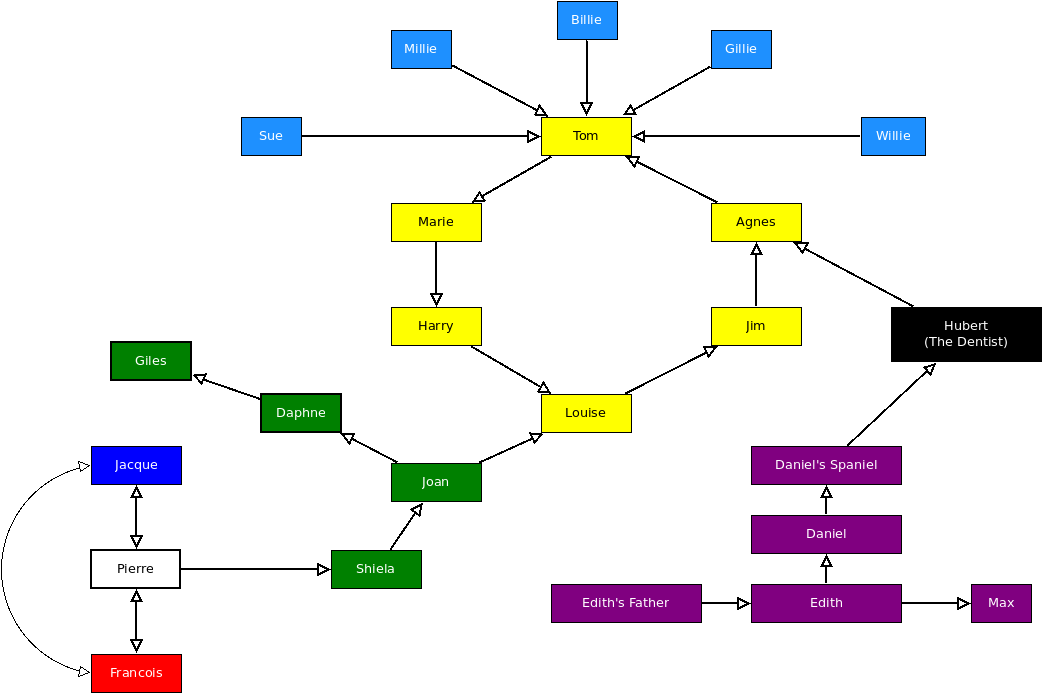
\includegraphics[scale=0.45]{Diagram3.png}
      \caption{ An example of how Endrun can be used by a small number of people.}
    \end{figure}
  
  Tom initiates a data transfer by generating an Endrun payload, and it gathers additional information at each node. Tom transferred the data to Marie, who transferred it to Harry, who provided it to Louise.
  
  Meanwhile, in France, Francois and Jacques compile some interesting information and then generate an Endrun payload for Pierre. Pierre grabs it via Sneakernet+, and then generates a payload for Sheila, who is visiting him in Paris.
  
  Louise wants to transfer data to Agnes. Louise transfers the data via Jim. Louise has additional data from Joan, who couriered a USB stick from Sheila (who is now in Ireland), and passed the data in turn to Daphne and Giles.
  
  Edith's father obtains some sensitive information and gives it to Edith for collation and cleanup. Edith then issues two endrun payloads, saves them to some spare SD cards she has lying around, and gives one copy each to Daniel and Max. Once Daniel returns home, he imports the payload into his personal Endrun node, generates a new payload for his dentist (who happens to be an intelligence operative), and saves it to a MicroSD card. Daniel then clandestinely places the card in the collar of his prize-winning spaniel, whom he takes to his dentist's appointment the next day.
  
  Agnes, who happens to be primary data coordinator in her circle of friends, then transmits the data to Tom, who also receives data from Sue, Millie, Billie, Gillie, and Willie. All of this data happens to be duplicate transmissions of the same payload.
  
  \section{Future Work}
  
  There are several features we would like to add to Endrun to fill out its capabilities. In addition, as a distributed, sequenced data storage and communications system, Endrun could be used to implement a wide variety of systems. We will detail two that we think are particularly compelling.
  
  \subsection{Additions to Endrun}
  
  \begin{itemize}
    \item \textbf{\textsc{Auditing}} - At the moment, the chain of custody can be used manually to trace the path a message took, and to debug problems in a transmission path. However, the chain is stored locally on each node and on each bundle, and so when bundles fail, it is currently labor-intensive to contact each node to find which processed a particular bundle. To rectify this, nodes could be configured periodically to send their lists of known bundles to a centralizer, which could perform traffic analysis after the fact. We have not yet implemented this, as there are significant security concerns about centralizing that level of audit logs, but there are use cases in which it would be helpful.
    
    \item \textbf{\textsc{Bluetooth Beaconing}} - Both iOS and Android provide for Bluetooth beacons (for Apple, they are called iBeacons) to identify locations and data sources; these beacons do not require pairing to communicate their (very short) messages, and correctly-programmed applications can use the beacons to trigger additional actions. We could add beacon functionality to native apps implementing the Sneakernet++ functionality we currently use, so that iOS and Android phones could receive a beacon, automatically connect to an Endrun node, download/upload bundles, and disconnect with little or no user interaction. This would allow Endrun nodes to be serviced by mobile platforms that may not have the time or capability for constant human interactions; for instance, mobile nodes could be attached to cars, bicycle couriers, or city buses.
  \end{itemize}
  
  \subsection{Best-Effort Surveillance}
  
  Current large-scale surveillance infrastructure is based around centralizing as much data as possible. Some proposals for increasing the scale of surveillance in major metropolitan areas include not only unprecedented government-installed camera density, but also integration of private cameras (e.g., from business surveillance cameras). Attempting to get real-time video from an increasing amount of cameras into a single location requires an extreme amount of data throughput---but this is an unnecessary action. Most alleged goals of widespread surveillance could be met with eventual data delivery, rather than immediate; therefore, we could extend Endrun to be used with cameras that will store data on nodes. Periodic collections, for instance, by mounting mobile Endrun nodes on city buses, could ``pick up'' the data and deliver it to centralized surveillance centers after some time, thus capturing the same data with more reasonable throughput needs.
  
  \subsection{Long-Distance Debt Instruments}
  
  In \emph{Neptune's Brood,} Charles Stross details a three-tiered system for interstellar currency, with ``fast money,'' ``medium money,'' and ``slow money'' describing progressively longer-term debt instruments. We believe that this concept, in conjunction with Endrun, could be used to create a system of debts and favors that could be traded between hackerspaces around the world, providing not just a way to identify key members of foreign hackerspaces (the so-called ``hackerspace passport'' concept), but a way for hackerspaces to help traveling members and have some ability to be repaid in turn. We hope to explore this idea in a future project.

\end{document}
